\subsection{IBM Spectrum Scale - GPFS}

Bei IBM Spectrum Scale handelt es sich um ein System, dass den gleichzeitigen Zugriff auf ein oder mehrere Dateisysteme zur Verfügung stellt von verschiedenen Knoten. Diesen können mithilfe von unterschiedlichsten Techniken den Zugriff zur Verfügung stellen (SAN, NAS, DAS) und ermöglichen das Aufsetzen von einem hochperformanten skalierbaren Netzwerkes \parencite[S. 1]{ibm.2017}.

Neben einfachen Datenzugriff werden ein Vielzahl von zusätzlichen Features geboten: Datei Duplizierung, Regel basiertes Speicher Management, Kommunikation und Zusammenschluss verschiedener Rechenzentren und diverse andere. Auf diese wird hier aber nur sehr grob eingegangen, da sie größtenteils unrelevant für die Arbeit sind und deren Umfang übersteigen würden.

\textbf{Hauptkomponenten und Funktionen}

Von jedem Knoten des Clusters kann gleichzeitig auf sämtliche Daten zugegriffen werden. Aufgrund der \gls{POSIX} Kompatibilität kann der Zugriff über Systemfunktionen (open, read, write) oder speziellen APIs erfolgen. Dies vereinfacht die Bedienung erheblich, da der Cluster für den einzelnen Rechner wie eine ``normale'' Festplatte erscheint. Auf jedem GPFS Knoten sind drei Hauptkomponenten installiert:

\begin{itemize}
	\item \textbf{GPFS Administration Kommandos} \\
	Eine Reihe von Skripts und Programme, die Konfigurationen ändern und Operationen auslösen können. Ausgeführte Kommandos können beliebige Knoten betreffen und werden entsprechend weitergeleitet und auf entfernten Systemen ausgeführt.
	\item \textbf{GPFS Kernel Erweiterung} \\
	Diese Erweiterung bietet ein Interface zum Betriebssystem und ermöglicht es GPFS als natives Dateisystem zu registrieren. Hierdurch erscheint der gesamte Cluster für eine Applikation wie eine einzelne Festplatte. Der Kernel führte diese entweder lokal auf verfügbarem Speicher aus oder leitet sie mithilfe des GPFS Daemon zu anderen Geräten weiter.
	\item \textbf{GPFS Daemon} \\
	Aufgabe dieses multithreaded Programmes ist das Ausführen sämtlicher Schreib-, Lese- und Pufferaktionen. Er sorgt auch für die Datenkonsistenz des Gesamtsystems. Zusätzlich zu den I/O Aktionen wird auch die Kommunikation mit anderen Knoten im System ausgeführt, um Konfigurationsänderungen, Wiederherstellung und parallele Updates durchzuführen.
	Ebenfalls enthalten ist die Network Shared Disk Komponente, die Cluster weite Benennung von und den Zugriff auf Speicher zur Verfügung stellt \parencite[S. 6]{ibm.2017}.  
\end{itemize} 

\textbf{Cluster Arten}

Es kann eine Vielzahl von Cluster Konfigurationen erreicht werden, da Spectrum Scale unterschiedlichste Betriebssysteme unterstützt (speziell Linux, AIX, Windows) und Speicher auf verschiedene Arten anschließbar ist. Im Folgenden werden zwei häufige Szenarien vorgestellt.

Eine Variante ist der Anschluss von sämtlichen Knoten an das selbe Storage Area Network. Ist dies nicht der Fall, können nur einzelne Nodes angeschlossen sein als \ac{NSD} Server und die verbleibenden sind \ac{NSD} Klienten. Hierbei wird eine klassische Server-Client Architektur aufsetzen bei der eine Vielzahl von GPFS Klienten auf eine kleinere Anzahl von GPFS Servern mit Speicheranbindung zugreift \parencite[S. 8]{ibm.2017}.

\begin{figure}[hbt]
	\centering
	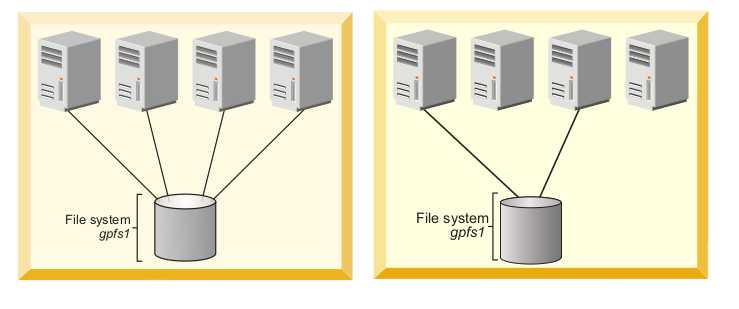
\includegraphics[scale=0.6]{images/gpfs-architectures}
	\caption{Anbindung an alle Knoten (links) und Server-Klient Architektur (rechts) \parencite[S. 8]{ibm.2017}}
	\label{fig:gpfsarchitecture}
\end{figure}

\textbf{Verbindung mit Cloud Diensten}

Cloud Dienste mit Spectrum Scale bieten zwei Funktionsweisen: \textbf{Cloud Tiering} und \textbf{Data Sharing}. Es können maximal vier verschiedene Knoten und ein Dateisystem für diese Dienste verwendet werden \parencite{mani.2017}.

Im ersten Szenario werden so genannte kalte Daten (also Dateien, die selten benutzt werden und geringe Zugriffszahlen haben) in der Cloud gespeichert, um die schnellen lokalen Datenspeicher zu entlasten. Dadurch kann die Clusterperformance erhöht und kosten für zusätzlichen Speicher gespart werden. Diese Funktion ist das Information Lifecycle Management (\ac{ILM}) System eingebunden und ermöglicht es den Administratoren Strategien zu definieren, um die Auslagerung bei bestimmten Daten auszulösen.
Es sollten nur kalte Files in der Cloud gespeichert werden, da diese bei Zugriff zu downloaden sind, was die Latenz massiv erhöht \parencite[S. 107]{ibm.2017}.
Lokal wird ein Cloud Verzeichnis angelegt, welches alle migrierten Daten auflistet. Wird auf einen Datei-Stub zugegriffen, kann die ferne Information heruntergeladen werden. In der Cloud liegen pro File zwei verschlüsselte Dateien, eins für die eigentlichen Daten und ein zweites mit Metadaten (Besitzer, Zugriff, ...) \parencite[S. 108]{ibm.2017}.

Beim Cloud Sharing ermöglicht das Teilen von lokalen Daten mit verschiedenen Arten von Objekt Speichern (\autoref{subsec:objectstorage}). Dieser Export kann ebenfalls durch IML Strategien in regelmäßigen Zyklen ausgelöst werden, um zum Beispiel Daten in der Cloud aktuell zu halten. Diese können dann von anderen Applikationen verwendet werden. Es ist ebenfalls ein Import von Object Storage System möglich, um die lokalen Daten ggf. zu erweitern.
Der Export wird parallel mit allen Cloud Dienst Knoten durchgeführt. Dabei kann eine Liste aller Daten in einem Manifest gespeichert werden, um diese später nachzuverfolgen.
Der größte Unterschied zur Migration beim Cloud Tiering ist, dass die Dateien in der Cloud nicht verschlüsselt werden, da sie auch für andere Nutzer verfügbar sein sollen und dass nach einem Transfer keine Verbindung (keine Updates bei späteren Änderungen) mehr zwischen lokalen und entfernten Files besteht \parencite[S. 109]{ibm.2017}.

Konfiguration dieser beiden Funktionalitäten kann mit dem \lstinline|mmcloudgateway| Programm vorgenommen werden \parencite{ibmadmin.2017}.

\subsection{Apache Hadoop - HDFS}

Apache Hadoop (ab hier nur noch Hadoop) ist ein Framework zu Entwicklung von massiven verteilten Systemen. Es ist in der Lage große Mengen von Daten, sowohl strukturiert wie auch unstrukturiert, über viele verteilte Berechnungsknoten zu verteilen und zu bearbeiten. Das Hauptsystem von Hadoop verwendet ein eigenes Dateisystem HDFS \parencite[Kap. I,1]{alapati.2016}.

Diese System sorgt für eine automatische Datenreplikation und unterstützt ebenfalls das leichte Hinzufügen von weiteren Servern mit zusätzlichen Diskstorage. Ein typischer Hadoop Cluster besteht aus Master- (hier läuft die Hadoop Software), Arbeiterknoten (Bereitstellung von Speicher mit HDFS und Rechenleistung mit \ac{YARN}) und so genannten Edge Servern (Zugriff auf den Cluster zum Ausführen von Programmen). Zusätzlich kann es noch Server für zusätzliche Frameworks geben und Datenbanken für spezielle Metadaten \parencite[Kap. I,1]{alapati.2016}.

Bearbeitung der Daten kann mithilfe verschiedener Anwendungsframeworks passieren, besonders beliebt ist hierbei MapReduce und Apache Spark.

Standardmäßig repliziert HDFS jeden Datensatz dreimal, um eine hohe Ausfalltoleranz zu garantieren. Es wird ein  write-once-read-many (\ac{WORM}) Zugriffsmodel verwendet, sodass Konsistenz kein Problem darstellt, da immer nur ein Nutzer auf eine Datei schreiben kann. Daten werden in große Blöcke (zum Beispiel 256 MB) aufgeteilt und auf verschiedenen Maschinen gespeichert. Hierdurch können auch sehr große Files gesichert werden, die für einzelne Maschinen zu viel Speicher verbrauchen würden. Metdaten für alle Blöcke werden innerhalb einer NameNode im RAM und auf konsistenten Speicher gespeichert  \parencite[Kap. I,2]{alapati.2016}.

Hadoop kann auch komplett in der Cloud verwendet werden, es gibt einige Hosting Anbieter (Amazon EC2, Google Computing Engine), die einen dynamischen Funktionsumfang zur Verfügung stellen \parencite[Kap. I, 1]{alapati.2016}.

\subsection{Google File System - GFS} \todo{Really wanna do that?}
\subsection{Objekt Dateisysteme} \label{subsec:objectstorage}

Objekt Speicher ist eine moderne Speicher Technologie und eine logische Weiterentwicklung von Block- oder Dateispeicher. Es soll Probleme von klassischen Lösungen wie komplexe Speicherhierachie, Defragmentierung von File Systemen, sowie Sicherheit und Zugriff umgehen.

\begin{figure}[hbt]
	\centering
	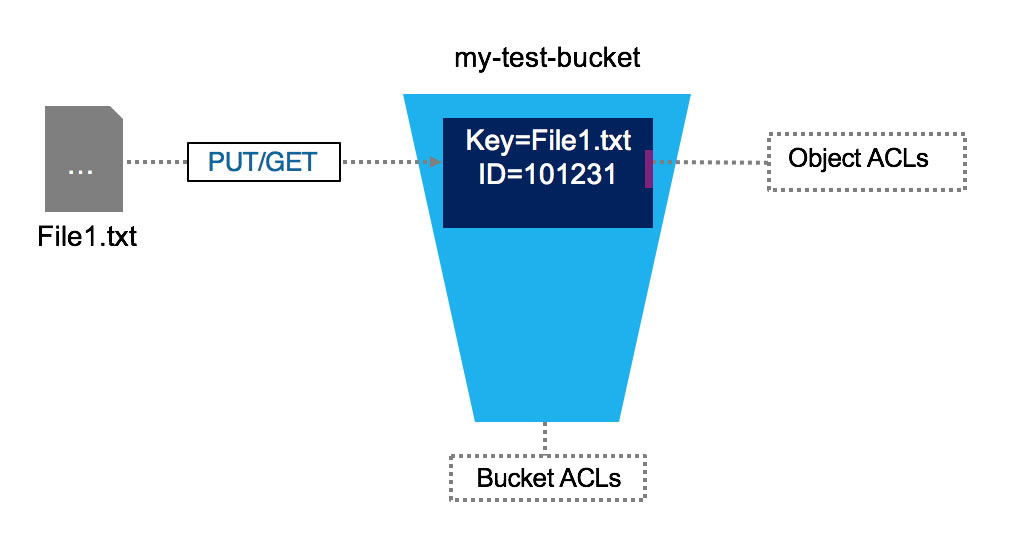
\includegraphics[scale=0.4]{images/object-storage}
	\caption{Komponenten von Objekt Speichern \parencite[S. 5]{Rios.2017}}
	\label{fig:objectstorage}
\end{figure}

Dieser Typ von Dateisystem umfasst drei Hauptkomponente:

\begin{itemize}
	\item \textbf{Daten:}\\
	 Nutzer und Anwendungsinformationen, die persistent hinterlegt werden müssen. Jede Art von Format ist hierbei unterstützt.
	\item \textbf{Metadaten:}\\
	 Diese sind Informationen über die eigentlichen Daten. Beispiele hierfür sind Dateigröße oder Uploadzeit. Ebenfalls können benutzerdefiniert Schlüssel-Wert Paare von nutzenden Anwendungen gespeichert werden. Diese sind von den Applikationen oder Usern zu jeder Zeit frei veränderbar. Eine Besonderheit dieses File Systems ist, dass die Metadaten zusammen mit den eigentlichen Daten gespeichert werden.
	\item \textbf{\ac{UUID}:} Diese eindeutige ID wird jedem Objekt im Speicher zugeordnet. Mit ihr können Daten unterschieden  und gefunden werden, unabhängig von der physikalischen Position der eigentlichen Informationen.
\end{itemize}

Durch obige Eigenschaften wird eine flache Hierarchie erzeugt, die Probleme mit außer Kontrolle geratenen Metadaten Speichern verhindert. Daten können in sogenannten Buckets zusammengefasst werden, um eine logische Strukturierung einzuführen und ebenfalls die Zugriffsrechte von Nutzern einschränken können.  

Da diese Art von Daten fast immer in der Cloud oder auf einem entfernen Server verwendet wird, bieten sich besonders REST Schnittstellen zum Zugriff auf die Daten an \parencite[S. 4f]{Rios.2017}.

\todo{Validate Information for other systems}
